\subsection{M-扭曲微分形式}

10.3.1. 设 X 是类 \(C^{r}\) 的实流形，M 是以 X 为底空间、有限秩且类 \(C^{k}\) 的向量丛，其中 \(0 \leqslant k \leqslant r\)。令 \(\lambda_{\mathrm{M}} = (\mathrm{Or}_{\mathrm{M}}, \{\pm 1\}, \mathrm{X}, \pi)\) 为与 M 的定向流形相关的主纤维化（10.2.2）。令结构群 \(\{\pm 1\}\) 通过乘法作用于 R。我们把 \(\tilde{R}_{M}\) 记作与 \(\lambda_{M}\) 相关的、纤维类型为 R 的丛（赋予上文定义的运算律）（6.5.1）；它带有（7.10.2）一个以 X 为底、秩为 1 且类 \(C^{k}\) 的向量丛结构；称为 M-扭曲标量丛。

10.3.2. 我们有一个交换图：

\pandocbounded{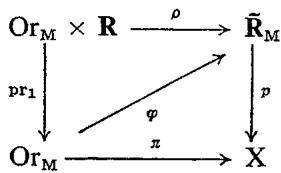
\includegraphics[keepaspectratio]{images/part001_9c73fb1b.jpg}}

其中 \(p\) 表示 \(\tilde{\mathbf{R}}_{\mathbf{M}}\) 到 \(\mathbf{X}\) 的典范投影，\(\rho\) 表示 \(\tilde{\mathbf{R}}_{\mathbf{M}}\) 的标架映射（6.5.1），并且有 \(\varphi(\xi) = \rho(\xi, 1)\)，其中 \(\xi \in \mathrm{Or}_{\mathbf{M}}\)。特别地，丛 \(\tilde{\mathbf{R}}_{\mathbf{M}}\) 在 \(\pi\) 下的逆像可与平凡丛 \(\mathrm{Or}_{\mathbf{M}} \times \mathbf{R}\) 等同。还将 \(\xi\)（\(\mathrm{Or}_{\mathbf{M}}\) 中的元素）与其在 \(\tilde{\mathbf{R}}_{\mathbf{M}}\) 中的像通过 \(\varphi\) 等同；按照这一约定，有 \(\rho(\xi, a) = a\xi\)（对所有 \((\xi, a) \in \mathrm{Or}_{\mathbf{M}} \times \mathbf{R}\)）；有 \(a\xi = b\eta\) 当且仅当存在 \(e \in \{\pm 1\}\) 使得 \(b = ea\) 且 \(\eta = e\xi\)。因此，\(\xi\) 是 \(\mathbf{M}\) 的一个定向，定义了截面 \(x \mapsto \xi(x)\)，它取值于 \(\tilde{\mathbf{R}}_{\mathbf{M}}\)。

存在唯一一个同构 \(j\)，它从 \(\tilde{\mathbf{R}}_{\mathbf{M}} \otimes \tilde{\mathbf{R}}_{\mathbf{M}}\) 到平凡丛 \(\mathbf{R}_{\mathbf{x}} = \mathbf{X} \times \mathbf{R}\)，使得 \(j(\xi \otimes \xi) = (\pi(\xi), 1)\) 对所有 \(\xi \in \mathrm{Or}_{\mathbf{M}}\) 成立；借此可将向量丛 \(\tilde{\mathbf{R}}_{\mathbf{M}}\) 与其对偶等同。

10.3.3. 设 F 还是以底空间 X 为基底、类 \(C^{r-1}\) 的向量丛。X 上取值于 \(\tilde{R}_{M} \otimes F\) 的微分形式称为取值于 F 的 M-扭曲微分形式。此类 p 次形式是丛 \(\operatorname{Alt}^{p}(\mathrm{T}(\mathrm{X}); \tilde{\mathbf{R}}_{\mathbf{M}} \otimes \mathbf{F})\) 的截面，并以显然的方式将其与 \(\tilde{R}_{M} \otimes \operatorname{Alt}^{p}(\mathrm{T}(\mathrm{X}); \mathbf{F})\) 等同。当 F 是由 Banach 空间 E 定义的平凡丛时，简称为取值于 E 的 M-扭曲形式；当 E = C（相应地 R）时，称为复 M-扭曲形式（相应地称为实 M-扭曲形式，或 M-扭曲形式）。

设 \(\omega\) 是取值于 F 的 M-扭曲形式，次数为 \(p\)。由于 \(\pi\colon\mathrm{Or}_{\mathbb{M}}\to\mathbf{X}\) 是 étale 的，且 \(\pi^{*}(\tilde{\mathbf{R}}_{\mathbb{M}})=\mathrm{Or}_{\mathbb{M}}\times\mathbf{R}\)，所以可以将 \(\pi^{*}(\tilde{\mathbf{R}}_{\mathbb{M}}\otimes\operatorname{Alt}^{p}(\mathrm{T}(\mathrm{X});\mathrm{F}))\) 与 \(\mathrm{Alt}^{p}(\mathrm{T}(\mathrm{Or}_{\mathbb{M}});\pi^{*}(\mathrm{F}))\) 等同，而 \(\omega\) 定义了 \(\tilde{\omega}\)（7.4.3）作为 \(\mathrm{Alt}^{p}(\mathrm{T}(\mathrm{Or}_{\mathbb{M}});\pi^{*}(\mathrm{F}))\) 的截面，换言之，是次数为 \(p\)、定义在 \(\mathrm{Or}_{\mathbb{M}}\) 上且取值于 \(\pi^{*}(\mathrm{F})\) 的微分形式。由此得到一个双射，从 X 上取值于 F 的 M-扭曲形式空间（次数为 \(p\)）到形式空间：其中 \(\tilde{\omega}\) 是次数为 \(p\)、定义在 \(\mathrm{Or}_{\mathbb{M}}\) 上且取值于 \(\pi^{*}(\mathrm{F})\) 的形式，且满足

\[
\tilde{\omega}(-\xi)=-\tilde{\omega}(\xi)\quad\text{对每个 }\xi\in\mathrm{Or}_{\mathbb{M}}.
\]

当 M 配备一个定向 \(\xi\) 时，映射 \(\omega \mapsto \xi \otimes \omega\) 使得可以将 \(\mathrm{Alt}^p(\mathrm{T}(\mathrm{X});\mathrm{F})\) 的截面（换言之，\(p\) 次通常微分形式）与取值于 F 的 \(p\) 次 M-扭曲形式等同。

10.3.4. 设 \(\omega\) 是 X 上取值于 Banach 空间 E、次数为 \(p\) 且类为 \(\mathbf{C}^s\) 的 M-扭曲微分形式（\(1 \leqslant s \leqslant \inf(k, r - 1)\)）。存在唯一一个 M-扭曲微分形式 \(d\omega\)，次数为 \(p + 1\)，取值于 E，且满足：对于 X 的每个开集 U、每个定向 \(\xi\)，属于 \(M|_{U}\) 的，以及 U 上的每个微分形式 \(\alpha\)，若 \(\omega|_{U} = \xi \otimes \alpha\)，则 \(d\omega|_{U} = \xi \otimes d\alpha\)。形式 \(d\omega\) 属于类 \(\mathbf{C}^{s-1}\)；称为 \(\omega\) 的外微分。

若将 \(\tilde{\omega}\)（相应地 \(\widetilde{d\omega}\)）记作 \(\mathrm{Or}_{\mathbb{M}}\) 上与 \(\omega\)（相应地与 \(d\omega\)）对应的微分形式，如 10.3.3 中那样，则有 \(d(\tilde{\omega}) = \widetilde{d\omega}\)。

若 \(\zeta\) 是类为 \(\mathbf{C}^s\) 的向量场，定义在 \(X\) 上，则以类似方式定义 M-扭曲形式 \(\theta_{\zeta}.\omega\)。有

\[
\theta_ {\zeta}. \omega = d (i (\zeta) \omega) + i (\zeta) d \omega
\]

并且 \(\theta_{\zeta}.\omega\) 属于类 \(\mathbf{C}^{s - 1}\)。

